\section{Implementation}\label{impl}

\begin{figure*}[tb]
\centering
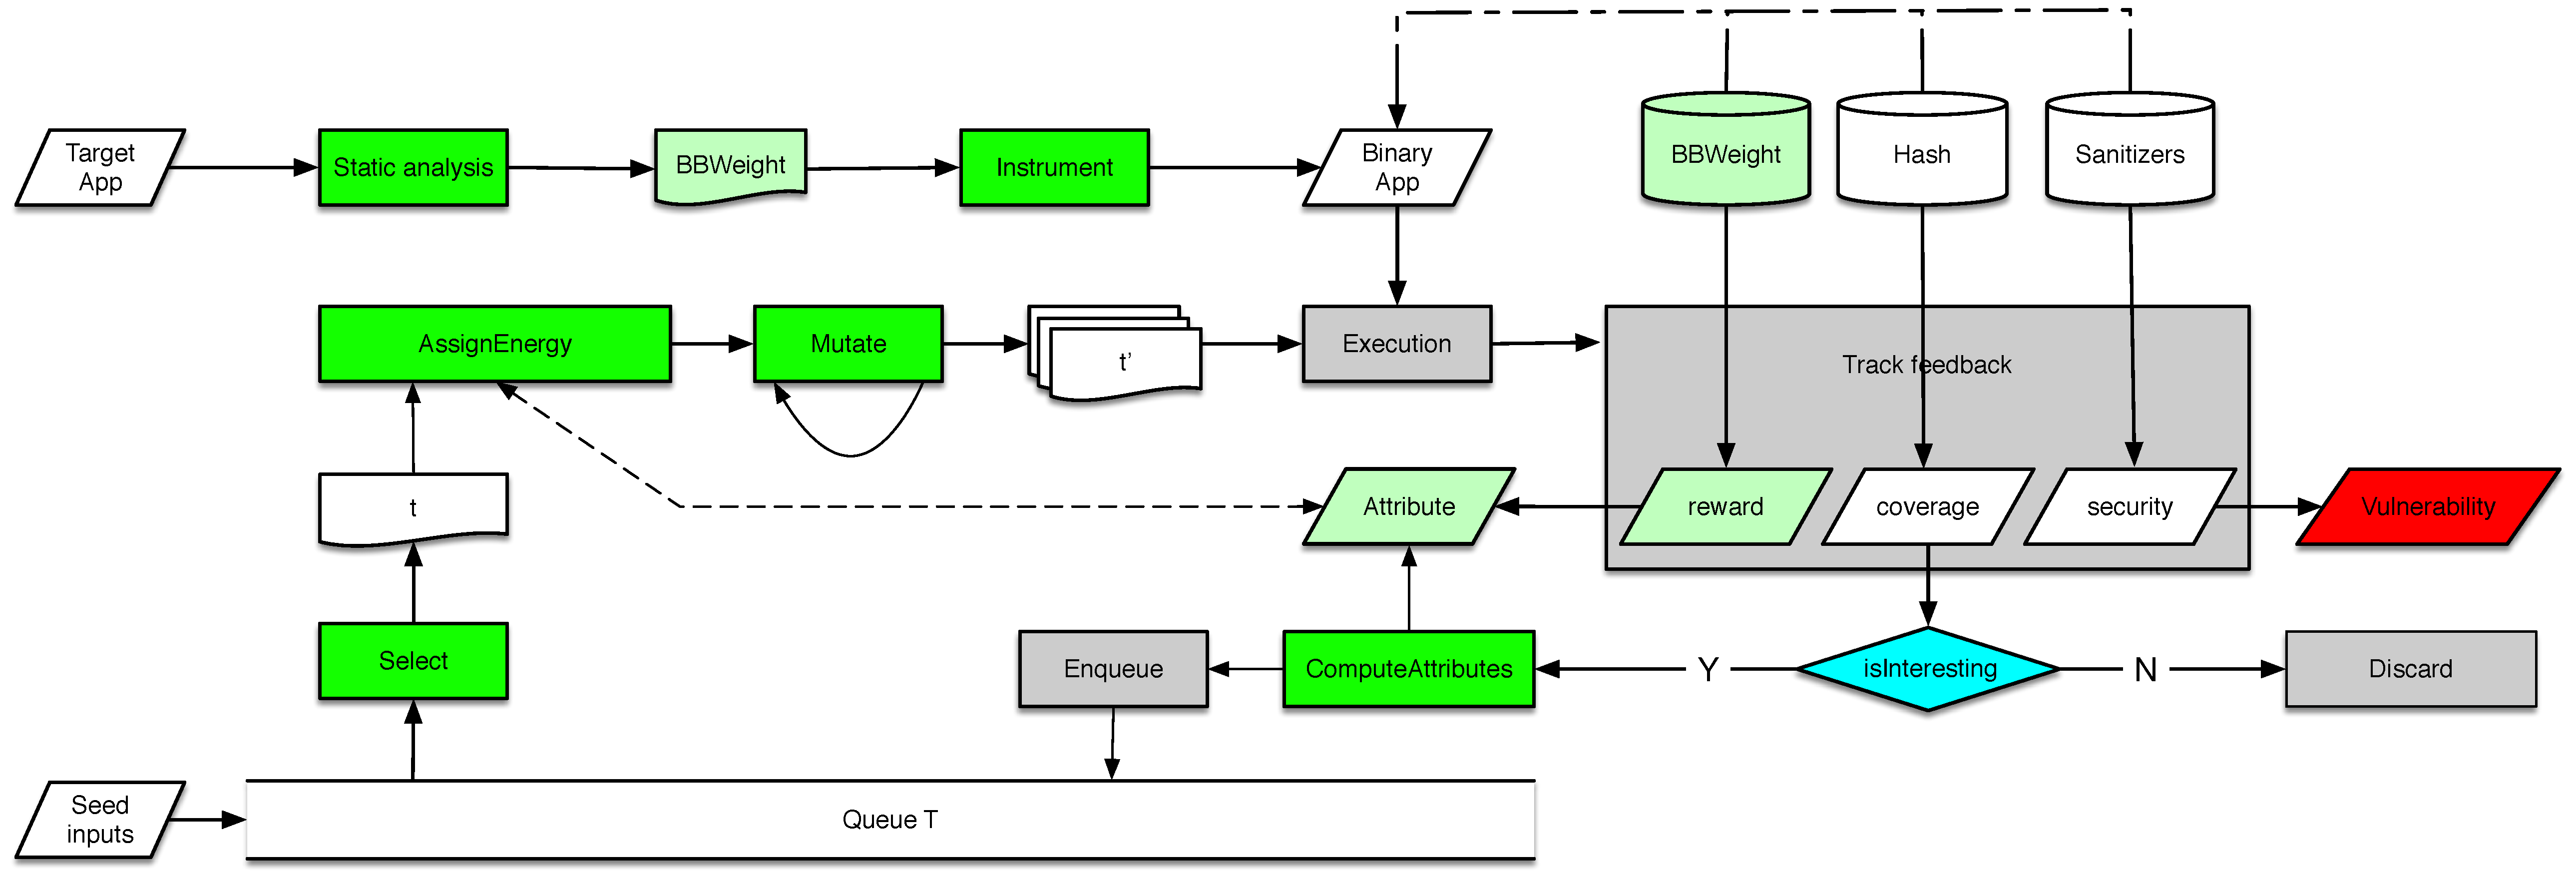
\includegraphics[width=7.2in]{pic/TAFL.eps}
\caption{Overview of TAFL}
\label{table:tafl}
\end{figure*}

We incorporate the aforementioned improvements into AFL's energy distribution, and developed a new fuzzing tool named TAFL on top of afl-2.52b. 

An overview of TAFL is illustrated in Fig. \ref{table:tafl}. Firstly, four kinds of promising vulnerable regions related metrics are extracted from a target program by static analysis. Then extracted weights of metrics are instrumented into target binary using compiler instrumentation. The reward of path exercised by a input was traced at run-time. These path rewards are used to distribute fuzzing energy, which includes phrases of selecting seed and assigning energy. TAFL prefers to select test cases that win higher rewards and assign more energy for them. The directed fuzzer strengthens fuzzing these promising vulnerable regions (i.e. sensitive regions, complex regions, deep regions and rare-reach regions). Furthermore, scheduling of mutation operators will increase the proportion of extra mutators over time, which have better ability to trigger new paths. The details of implementation are described in the following:

\subsubsection{Metric  Extraction}
Weight extraction for each metric is implemented as one LLVM pass \cite{pass}. They are used to obtain weight value of region's feature related metrics including sensitive degree, complexity, depth and rare-reach degree. These passes are used and activated by compiler afl-clang-preprocess. Each preprocess pass has a corresponding environment variable, i.e., GET\_MEM\_DENSITY, GET\_INST\_NUM, GET\_DEPTH, and GET\_ENTRY\_DEGREE. When environment variable of compiler CC is set to afl-clang-preprocess, and any of above LLVM passes' environment variable is set, related weight information of each basic block is generated and stored into a text file after the project is built.

\subsubsection{Compiler Instrumentation}
The BB weight file for each metric consists of the BB's name and its metric weight value. It is taken by compiler to instrument the weight value into target executable binary. More specifically, an extended trampoline is injected for each basic block. The trampoline is a piece of assembly code that is executed after the jump instruction, in order to keep track of the coverage control-flow edges. An edge is represented by a byte in a 64KB shared memory. On a 64-bit architecture, we extend 16 additional bytes of shared memory to record the reward feedback. 8 bytes are used to accumulate weight value, and another 8 bytes are used to record number of executed basic blocks. The instrumentation is implemented as an extension of AFL LLVM pass. When performing instrumentation, set compiler to afl-clang-fast, and compiler's flags to reference related BB weight file, then build target project.

\subsubsection{Energy Distribution}
TAFL fuzzes the instrumented executable binary with integrated energy distribution strategy. It selects seed and assigns energy based on run-time reward of test case. The current test case's reward is computed by dividing accumulated BB weight for different metrics by the number of exercised basic blocks. TAFL selects those test cases that wins higher reward and assign energy based on seed's reward factor. Besides, its implementation of MutateInput in havoc stage is modified to improve the proportion of extra mutators over time.

We have open sourced our tool which is available for download at \url{https://sites.google.com/view/tafl/tool}.